\section{Storage e Audit Trail}
\label{sat}

\subsection{Backup dati}

Diverse aziende al giorno d'oggi sviluppano diverse milioni di linee di codice, 
e raggruppano queste linee in librerie, che vengono salvate nei sistemi. La 
perdita di queste liberie costituiscono una catastrofe. È quindi necessario:
\begin{itemize}
 \item Mantenere i backup dei dati lontani dall'azienda (off-site)
 \item Avere un posto sicuro in cui tenere le librerie/siti. Se questi siti 
 hanno informazioni sensibili è meglio tenerlo in un posto nascosto, la cui 
 conoscenza è ristretta a pochi.
\end{itemize}

\subsection{Audit Trail}

Chi fa cosa quando?

Fare audit non è una cosa semplice, ed è necessario seguire alcune 
\textit{best-practices}.

\begin{itemize}
 \item L'audit trail traccia le responsabilità (chi ha fatto cosa e quando?). 
 Il concetto è quello di utilizzare il tracciamento continuo, in modo da poter 
 capire quali sono le cause che hanno generato l'evento negativo
 \item Il log deve essere sicuro, l'attaccante potrebbe penetrare il sistema, 
 ottenere una topologia della rete, attaccare il servizio, accedere ai dati e 
 cancellare le tracce dell'intrusione. I log devono essere sicuri (es. read 
 only). Un altro possibile attacco è alterare il timestamp dei log.
 \item Un'altra cosa importante per le grosse società con responsabilità verso 
 terzi è che i log siano firmati digitalmente.

\end{itemize}

\subsubsection{Strumenti per l'audit trail}

Sono presenti solitamente un sacco di informazioni catturate, che necessitano 
di essere distinte e categorizzate.
Una buona pratica è scremare l'informazione fin dall'inizio, e viene detto 
\textbf{audit reduction}.

È fondamentale essere in grado di trovare \textbf{varianze o cambiamenti 
anomali nel comportamento del sistema}. Esistono strumenti in grado di fare 
ciò, che mandano un allarme quando notano un'anomalia al di sopra del 
\textit{treshold}\footnote{Rappresenta la tolleranza che il sistema ha.} 
impostato. Recentemente si sta utilizzando l'intelligenza artificiale per 
risolvere questo tipo di problema.

\subsection{Esercizi}

Gli esercizi sono disponibile alla sezione \ref{EsSat}


\part{Networking}

\label{net}

\chapter{Network Security}

\section{The problem of Network Security}

Ci sono due punti fondamentali al giorno d'oggi:

\begin{itemize}
\item gli oggetti sono sempre connessi
\item ci saranno sempre più oggetti connessi
\end{itemize}

Negli ultimi anni si ha una pressione del mercato molto forte, e questo causa 
che la sicurezza dei sistemi non sia tenuta in adeguata considerazione. Si 
stima che nel mercato ci saranno 20 miliarti di dispositivi \textit{IoT}. 
Questo grande numero è anche dettato dal fatto che ``chi prima arriva meglio 
alloggia'', e quindi il primo che ha una buona idea riesce a prendersi la 
fascia maggiore di mercato. Gli utenti poi tenderanno a non cambiare più 
servizio (fenomeno chiamato come \textit{lock-in}). Un altro fenomeno 
importante è legato all'\textit{effetto scala}: è quando si esegue un gran 
lavoro per creare una nuova invenzione, per ottenere infine un guadagno minimo.

% Boh? Chissà cosa voleva dire il prof qui
%Il fattore scalabilità è molto importante anche. Quindi il fattore di scala 
%sulla network security è molto importante.

\section{Hacking networks}

Gli attacchi informatici si suddividono in diverse fasi, ognuna delle quali 
esegue un passo verso l'ottenimento dell'accesso fraudolento alle informazioni 
di un sistema.

% TODO trovare il nome della prima fase
\subsection{Fase 1: ?}\todo{Trovare il nome della prima fase}

Nella prima fase si cercano informazioni sulla vittima, e i posti migliori dove 
guardare sono:
\begin{itemize}
 \item accesso fisico
 \item guardare dentro i rifiuti dell'azienda per trovare informazioni
 \item recuperare informazioni da google, newsgroups web sites
 \item social engineering
 \item whols database \& arin.net
 \item interrogazioni al DNS
\end{itemize}

\subsection{Fase 2: \textit{Scanning}}

Soprattutto utile per le reti wireless. Per definizioni le reti wireless fanno 
\textbf{beaconing}: dichiarano le loro informazioni a tutti, e questo presenta 
delle falle di sicurezza. Sono presenti attacchi al giorno d'oggi noti e con 
percentuale fortissima di successo, così forte che se fossero applicate al 
\textit{wired} nessuno pagherebbe più online, per esempio.

\begin{itemize}
\item War driving: posso trovare una rete wireless?
\item War dialing: posso trovare un modem a cui connettermi?
\item Network mapping: ho qualcuno che esporta un servizio, quale servizio 
viene fornito su qualche porta?
\item Vulnerability-Scanning Tools: quale versione del software è installato 
sui dispositivi?
\end{itemize}

\subsubsection{Attacchi passivi}

Gli attacchi sono passivi quando l'attaccante agisce in maniera passiva, e non 
modifica il sistema (per esempio non cambia i dati all'interno dei pacchetti o 
cosa del genere). Un attacco passivo potrebbe essere per esempio catturare 
tutti i dati presenti all'interno del sistema. Questo tipo di attacco è 
disponibile anche sulle reti cablate, il problema che nelle reti cablate è 
possibile trovare se uno sta eseguendo questa azione.

\begin{itemize}
\item Eavesdropping: ascoltare pacchetti provenienti da altre parti (sniffing)
\item Traffic analysis: acquisire conoscenza sulla rete osservando i pattern di 
traffico
\item Footprinting: testare per determinare il software installato sui sistemi 
(network mapping)
\end{itemize}

\subsubsection{Attacchi attivi}

Gli attacchi sono attivi quando l'attaccante agisce in maniera attiva, per 
esempio modificando il contenuto dei pacchetti.

Questi sono una lista di attacchi attivi più famosi:
\begin{itemize}
\item DoS\footnote{DoS sta per \textit{Denial of Service}}
\item Masquerading of spoofing
\item Modificare il messaggio: il messaggio viene modificato durante la 
trasmissione. È sufficiente criptarlo.
\item Packet replay: un pacchetto viene ritrasmesso per accedere ad un servizio.
\end{itemize}

\subsection{Fase 3: Guadagnare l'accesso}

Quando si hanno sufficienti informazioni riguardo la vittima è possibile da 
parte dell'attaccante iniziare un attacco.
Attacchi alle reti che vengono solitamente perpetrati sono:

\begin{itemize}
\item sniffing
\item ip address spoofing
\item session hijacking
\end{itemize}

Attacchi al sistema:

\begin{itemize}
\item buffer overflow
\item password cracking
\item SQL Injection
\item abuso del protocolli web
\item DoS
\item Trap Door
\item virus, worm, trojan horse
\end{itemize}

\subsubsection{Attacchi}

\paragraph{Man-in-the-Middle Attack}

Il suo attacco si basa sullo scambio di chiavi tramite l'algoritmo di 
\textit{diffie-hellman}.

\subparagraph{Diffie-Hellman Key exchange protocol}

Inventato nel 1976, usa una crittografia a chiave asimmetrica.

Permette a due comunicanti di generare una chiave simmetrica senza basarsi su 
un segreto pre-definito (attenzione: non è un algoritmo di criptazione). 
Purtroppo sarà poco effettivo contro il quantum computing, ed è quindi cercare 
una soluzione alternativa prima dell'uscita del quantum computing.


\subparagraph{Secure Key generation}

Alice e Bob vogliono scambiarsi una chiave ma sono geograficamente lontani.

Le due parti si scambiano delle informazioni pubbliche. Queste informazioni 
vengono combinate con delle informazioni private per generare una chiave, 
utilizzata per l'\textit{encryption}.

\subsubparagraph*{Come avviene lo scambio dell'informazione pubblica e privata}

Vengono eseguiti i seguenti passi:

\begin{enumerate}
 \item Si sceglie un numero primo $p$ di grandezza ragionevole (almeno 2048 
 bit).
 \item Si prende una radice primitiva (generatore) di $p$: dato p prendo un 
 numero a caso, se ho un generatore so che esite un numero per cui elevando il 
 generatore a quel numero posso ottenere tutto il campo.
\end{enumerate}

\subsubparagraph*{Generazione della chiave simmetrica}
\todo{Da rivedere}

Parte privata: Alice genera un numero $x$, Bob crea un $y$, entrambi lo tengono 
segreto.

Alice: $R_1 = g^x mod\ p$
Bob: $R_2 = g^y mod\ p$

Queste informazioni vengono scambiate su un canale pubblico.

Bob riceve G1, quello che fa è fare $K = (R_1)^y mod\ p$. Alice fa la stessa 
cosa e quindi ottengono una chiave segreta condivisa che è $g^{xy} mod\ p$.

Il calcolo del logaritmo discreto ad oggi è un problema che è difficile da 
risolvere in maniera efficiente, ed è quello su cui la sicurezza si basa su 
questo problema.

\subparagraph{Esecuzione dell'attacco MITM}

Questo tipo di attacco è attivo, dove i dati vengono dirottati da un attaccante 
che sta nel mezzo dell'attacco, simulando una falsa trasparenza. Questa 
mediazione non è individuabile da parte dei due comunicanti legittimi. In 
questa maniera l'attaccante ha la possibilità di generare le chiavi per 
comunicare con Alice e Bob (i due comunicanti legittimi), ma lo fanno con 
l'attaccante nel mezzo, che è in grado di leggere tutte le comunicazioni.
L'attacco viene eseguito in questa maniera:
\begin{enumerate}
\item Viene mandato un messaggio da Alice
\item L'attaccante decripta il messaggio, lo salva e lo ricripta con la chiave 
simmetrica che usa da Bob e gli manda il messaggio
\item Bob legge il messaggio, senza sapere nulla.
\end{enumerate}


\subparagraph{Conclusioni}

DH è il cornerstone della sicurezza, viene usato quotidianamente. Non è un 
algoritmo di \textit{encryption}.
Per risolvere il problema dell'attacco è necessario aggiungere un meccanismo di 
autenticazione.

\paragraph{SQL Injection}

Sfrutta il fatto che ciò che viene passato come input che deve essere 
interpretata in un certo modo viene forzata ad essere interpretata in un altro.

Il modo migliore per proteggersi da questo tipo di attacco è di eseguirne un 
corretto \textit{escaping}.

\paragraph{Password cracking}

\begin{figure}[h!]
	\begin{center}
		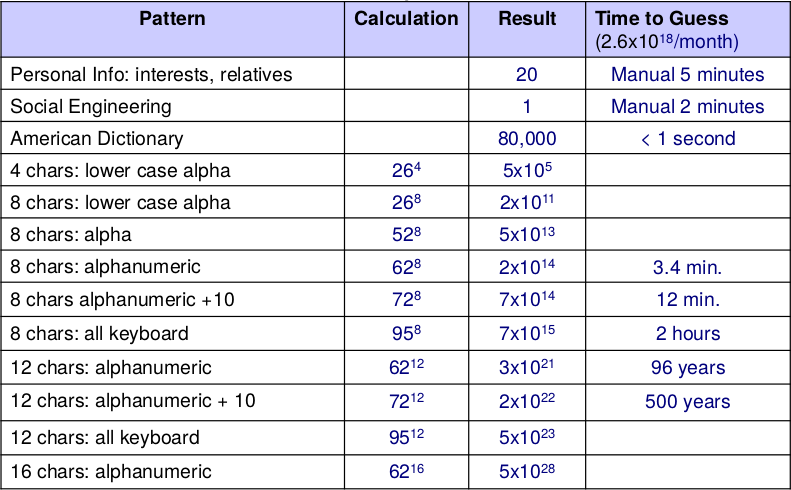
\includegraphics[scale=0.65]{res/img/password_cracking_table.png}
	\end{center}
	\caption{Tabella che mostra i più comuni pattern di password e il tempo necessario per violarli.}
	\label{fig:password:cracking:table}
\end{figure}

8 caratteri è il minimo per un password ed è anche poco, infatti in due ore è possibile 
rompere una qualsiasi password di 8 caratteri come mostra la tabella \ref{fig:password:cracking:table}.
